\chapter{RTS AI: \textit{StarCraft: Broodwar}}

\section{How does the game works: gameplay}
Really, the best is to play it... But I'll explain it.

In combinatorial game theory terms, competitive StarCraft is a zero sum, partial-information, deterministic strategy game.

\section{Problems, resolutions}

\begin{figure}[!ht]
\begin{center}
\begin{tikzpicture}
  \path[mindmap,concept color=black!80!white,text=white]
    node[concept] {RTS AI: predict, decide, perform}
    [clockwise from=-30]
    child[concept color=orange!90!black] {
      node[concept] {Micro}
      child[concept color=red!80!magenta] { node[concept] {React} }
      child { node[concept] {Optimize} }
      child[concept color=blue!80!cyan] { node[concept] {Cooperate} }
    }
    child[concept color=cyan!90!black] { % TODO change color
      node[concept] {Tactics}
      child[concept color=red!80!magenta] { node[concept] {When?} }
      child { node[concept] {Where?} }
      child[concept color=blue!80!cyan] { node[concept] {How?} }
    }
    child[concept color=green!70!black] {
      node[concept] {Strategy}
      child[concept color=red!80!magenta] { node[concept] {Aggressivity} }
      child { node[concept] {Spendings balance} }
      child[concept color=blue!80!cyan] { node[concept] {Army composition} }
    };  
\end{tikzpicture}
\end{center}
\label{fig:mindmapRTS}
\caption{A mind-map of RTS AI XXX TODO}
\end{figure}

\section{Task decomposition and linking}
\begin{figure}[!ht]
\begin{center}
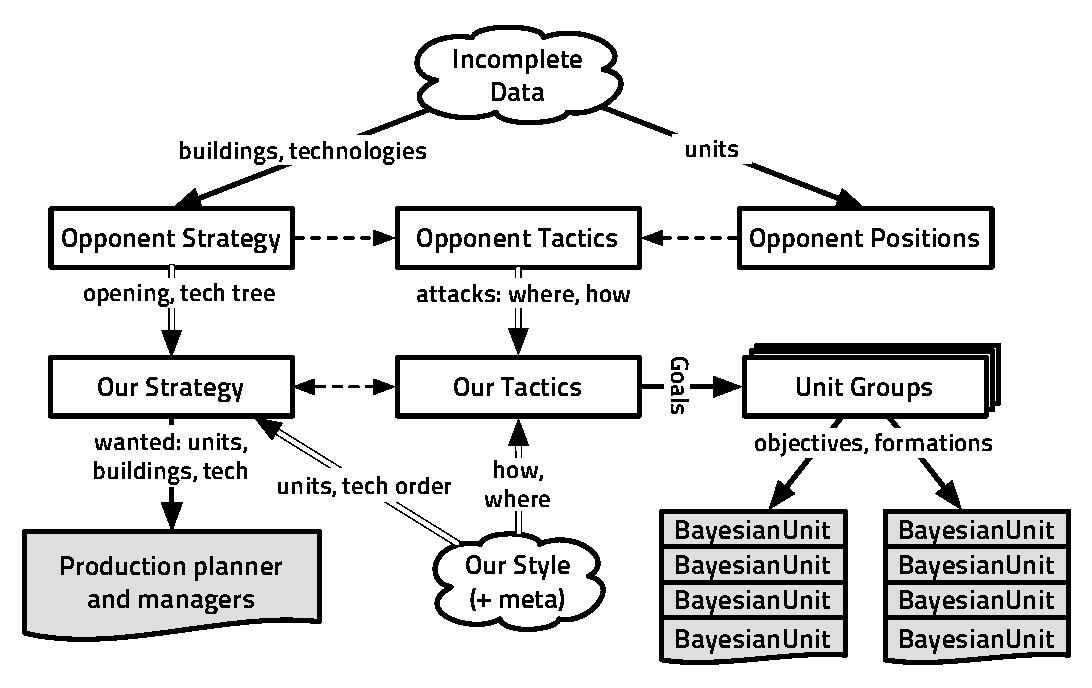
\includegraphics[width=13cm]{images/starcraft_bbq_concept.pdf}
\end{center}
\label{fig:conceptbbq}
\caption{Information-centric view of the architecture of the major components of the bot. Arrows are labeled with the information or orders they convey: dotted arrows are convey constraints, double lined arrows convey distributions, plain and simple arrows convey direct information or orders. The gray parts perform game actions (as the physical actions of the player on the keyboard and mouse).}
\end{figure}

In Fig.~\ref{fig:conceptbbq}, we present the flow of informations between the different inference and decision-making parts of the bot architecture. One can also view this problem as having a good model of one's strategy, one's opponent strategy, and taking decisions. The software architecture that we propose is to have services building and maintaining the model of the enemy as well as our state, and decision-making modules using all this information to give orders to actuators.

\begin{itemize}
\item Problem: build a real-scale software piece which is maintainable
\item State of the art: shared memories, shared states
\item Our take: we transmit distributions, states stay in modules
\item Results: XXX (atm too much state), also competitions results
\end{itemize}

% XXX 
XXX Real-time strategy (RTS) gameplay consist in producing and managing group of units with attacks and movements specificities in order to defeat an enemy. Most often, it is required to gather resources and build up an economic and military power while expanding a technology tree. Parts of the map not in the sight range of the player's units are under \textit{fog of war}, so the player only has partial information about the enemy buildings and army. The way by which we expand the tech tree, the specific units composing the army, and the general stance (aggressive or defensive) form what we call \textit{strategy}. At the lower level, the actions performed by the player (human or not) to optimize the effectiveness of its units is called \textit{micro-management}. In between lies \textit{tactics}: where to attack, and how. A good human player takes much data in consideration when choosing: are there flaws in the defense? Which spot is more worthy to attack? How much am I vulnerable for attacking here? Is the terrain (height, chokes) to my advantage? etc.

%TACTICS: We worked on StarCraft: Brood War, which is a canonical RTS game. It had been around since 1998, sold 10 millions licenses and reigned on competitive RTS for more than a decade. StarCraft (like most RTS) has a mechanism, \textit{replays}, to record every player's actions such that the state of the game can be deterministically re-simulated. Numerous international competitions and professional gaming (mainly in South Korea) produced a massive amount of data of highly skilled human players, performing about 300 actions per minute while following and adapting their strategies. In StarCraft, there are two types of resources, often located close together, minerals (at the base of everything) and gas (at the base of advanced units and technologies). There are 3 factions (Protoss, Terran and Zerg) which have workers to gather resources, and all other characteristics are different: from military units to ``tech trees'', gameplay styles.
